\documentclass[oneside, a4paper]{article}

\usepackage[left=25mm, right=25mm, top=25mm, bottom=25mm, paper=a4paper]{geometry}
\usepackage[utf8]{inputenc}
\usepackage[spanish]{babel}
\usepackage{csquotes}
\usepackage{float}
\usepackage{hyperref}
\usepackage{tabularx}
\usepackage{array}
\usepackage{graphicx}
\usepackage{fancyhdr}
\usepackage{amsmath}
\usepackage{multicol}
\usepackage[sorting=none, style=apa]{biblatex}

\graphicspath{{./../img/}}
\fancyhf{}
\fancyhead[L]{
\includegraphics[scale=0.15]{espe.png}}
\fancyhead[R]{
\includegraphics[scale=0.05]{ciencias_de_computacion.jpg}}
\setlength{\headheight}{50pt}
\setlength{\parindent}{0pt}
\addbibresource{bibliography.bib}
\emergencystretch=1em

\title{
    \Large
    \begin{center}
        \includegraphics*[scale=0.3]{espe.png}
    \end{center}
    \textbf{UNIVERSIDAD DE LAS FUERZAS ARMADAS ESPE}\\
    \textbf{DEPARTAMENTO DE CIENCIAS DE LA COMPUTACIÓN}\\
    \textbf{INGENIERÍA DE SOFTWARE}
}
\author{\\
    \textbf{NRC:} 14774\\
    \textbf{Materia:} Computación Gráfica\\
    \textbf{Tema:} Aplicaciones de Computación Gráfica\\\\
    \textbf{Grupo 2}\\
    Albán Richard\\
    Escobar Aymé\\
    Guacán Alexander\\
    Macas Karol\\\\\\\\
    Ing. César Javier Villacís Silva
}
\date{}

\begin{document}
    \pagestyle{fancy}

    \begin{titlepage}
        \maketitle
    \end{titlepage}

    \section{Descripción del problema}
        Escriba un programa para dibujar un panal de abejas, como se muestra en la Figura \ref{fig:bee_panel_example}. Para dibujar esta figura se debe leer el valor del lado de un hexágono como, por ejemplo: lado igual a 2. Se recomienda encerrar la figura dentro de un rectángulo y realizar los cálculos de los segmentos que encierran a la figura para poder graficarla.

        \begin{figure}[H]
            \centering
            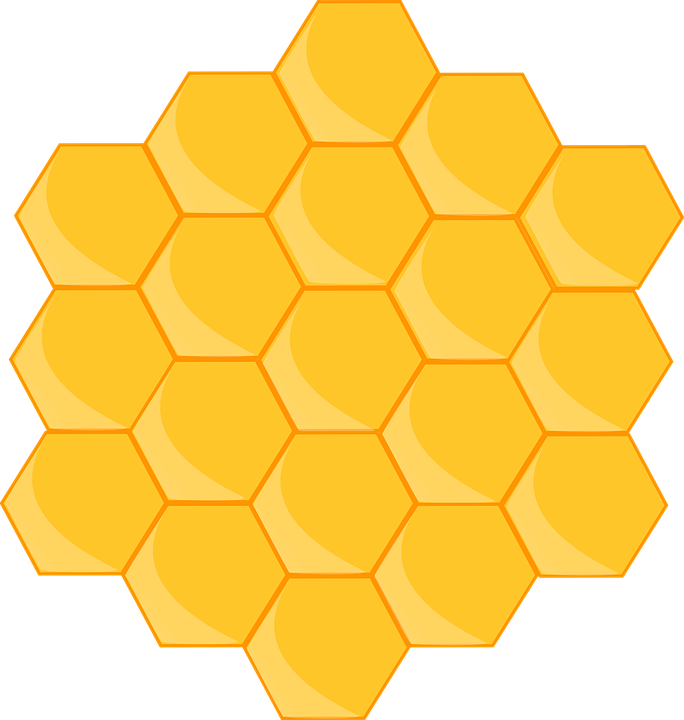
\includegraphics[scale=0.2]{bee_panel_example.png}
            \caption{Panel de abejas (\cite{bee_panel_example}).}
            \label{fig:bee_panel_example}
        \end{figure}

    \section{Geometría de la figura}
        \subsection{Hexágono}
            Para graficar el panal de abejas completo, primero debemos poder graficar un hexágono. Para ello debemos saber que un hexágono se construye usando triángulos equiláteros como puedes observar en la Figura \ref{fig:hexagon}, por lo que como dato principal sabemos que $\theta = 60^{\circ} $, además se ha encerrado al hexágono en un rectángulo , el cual representa el marco donde dibujaremos la figura, donde el centro de la misma, es el centro de este marco de dibujo.

            \begin{figure}[H]
                \centering
                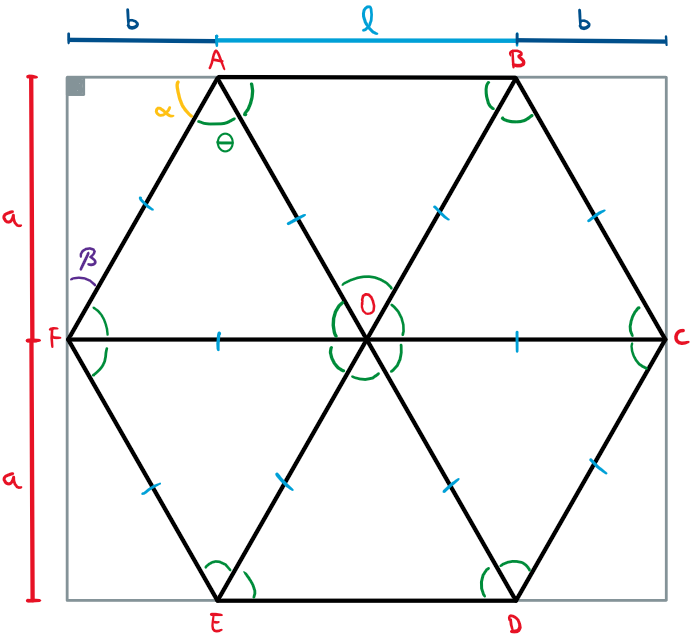
\includegraphics[scale=0.45]{hexagon.png}
                \caption{Vertices y lados del hexágono.}
                \label{fig:hexagon}
            \end{figure}

            Calculamos los ángulos del triángulo rectángulo exterior al hexágono:

            \begin{align*}
                2\theta + \alpha & = 180         & \alpha + \beta & = 90      \\
                \alpha           & = 180 - 2(30) & \beta          & = 90 - 60 \\
                \alpha           & = 60          & \beta          & = 60
            \end{align*}

            Utilizamos identidades trigonómetricas en el triángulo externo (Figura \ref{fig:external_triangle_rectangle}) para obtener el valor de la apotema del hexágono ($a$) y de la distancia de la esquina superior izquierda del marco de dibujo a el vertice $A$.

            \begin{figure}[H]
                \centering
                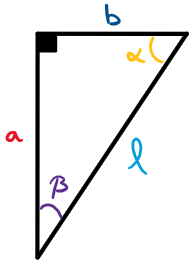
\includegraphics[scale=0.45]{external_triangle_rectangle.png}
                \caption{Triángulo externo al hexágono.}
                \label{fig:external_triangle_rectangle}
            \end{figure}

            \begin{multicols}{2}
                \begin{align}
                    \sin(\alpha) & = \frac{a}{l} \nonumber                          \\
                    a            & = l * \sin{60} \nonumber                         \\
                    a            & = \frac{\sqrt{3}}{2}l \label{eq:apothem_hexagon}
                \end{align}
                \begin{align}
                    \sin(\beta) & = \frac{b}{l} \nonumber                          \\
                    b           & = l * \sin{30} \nonumber                         \\
                    b           & = \frac{l}{2}  \label{eq:base_external_triangle}
                \end{align}
            \end{multicols}

            Por lo tanto, si ubicamos cada uno de los vertices con respecto al vertice central $O$ del hexágono, obtenemos:

            \begin{equation}
                \begin{aligned}
                    O(x, y) & = O(x_{O}, y_{O})         \\
                    A(x, y) & = A(x_{O} - b, y_{O} - a) \\
                    B(x, y) & = B(x_{O} + b, y_{O} - a) \\
                    C(x, y) & = C(x_{O} + l, y_{O})     \\
                    D(x, y) & = D(x_{O} + b, y_{O} + a) \\
                    E(x, y) & = E(x_{O} - b, y_{O} + a) \\
                    F(x, y) & = F(x_{O} - l, y_{O})
                \end{aligned}
                \label{eq:hexagon_vertices}
            \end{equation}
                
            Hay que aclarar que el punto $O(x_{O}, y_{O})$ es un punto dinámico, esto ya que cada hexágono del panal de abejas tendrán el mismo tamaño, pero lo que cambia es el centro desde el cual se comienza a dibujar.

        \subsection{Panal de abejas}
            Una vez que aprendimos a graficar los hexágonos que conforman el panal de abejas, procederemos a determinar los centros de cada uno de ellos. Lo primero que haremos es dividir al panal por columnas, en cada una de ellas necesitaremos una cantidad diferente de hexagonos como se puede observar en la Figura \ref{fig:bee_panel}.

            \begin{figure}[H]
                \centering
                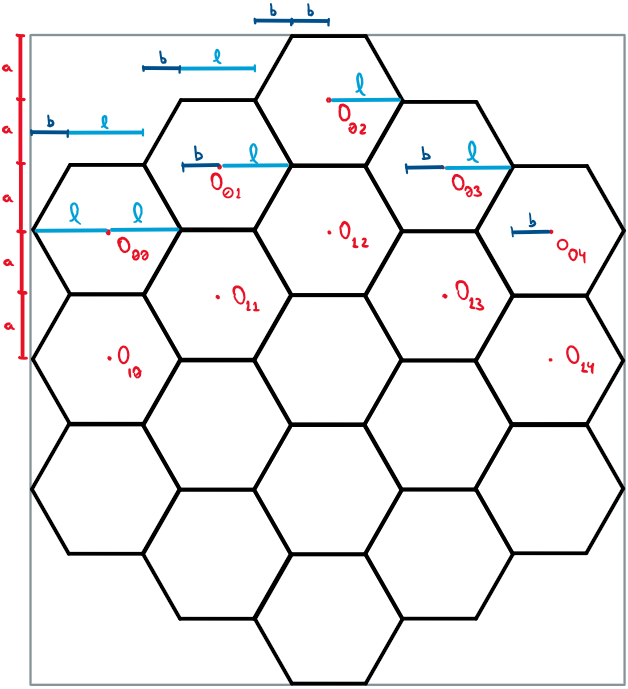
\includegraphics[scale=0.45]{bee_panel.png}
                \caption{Panal de abejas con medidas.}
                \label{fig:bee_panel}
            \end{figure}

            Si tabulamos los hexágonos a dibujar por columna obtenemos que:

            \begin{center}
                \begin{tabular}{ | c | c | }
                    \hline
                    
                    \textbf{Columna ($c$)} & \textbf{Hexágonos ($h$)} \\
                    
                    \hline
                    
                    0                      & 3                        \\
                    1                      & 4                        \\
                    2                      & 5                        \\
                    3                      & 4                        \\
                    4                      & 3                        \\

                    \hline
                \end{tabular}
            \end{center}

            Por lo tanto, la formula que nos permite determinar la cantidad de hexágonos a graficar por columna es:

            \begin{equation}
                h = - | c - 2 | + 5
                \label{eq:compute_hexagons_by_column}
            \end{equation}

            Al tabular cada uno de los centros de los hexágonos del panal de abejas, podemos encontrar un patrón:

            \begin{center}
                \begin{tabular}{ | c | c | c | c | c | c | }
                    \hline
            
                    $O_{ij}(x, y)$ & $0$              & $1$                   & $2$                    & $3$                    \\
            
                    \hline
            
                    $0$            & $(l, 3a)$        & $(2l + b, 2a)$        & $(3l + 2b, a)$         & $(4l + 3b, 2a)$        \\
                    $1$            & $(l, 5a)$        & $(2l + b, 4a)$        & $(3l + 2b, 3a)$        & $(4l + 3b, 4a)$        \\
                    $2$            & $(l, 7a)$        & $(2l + b, 6a)$        & $(3l + 2b, 5a)$        & $(4l + 3b, 6a)$        \\
                    $n$            & $(l, (2i + 3)a)$ & $(2l + b, (2i + 2)a)$ & $(3l + 2b, (2i + 1)a)$ & $(4l + 3b, (2i + 2)a)$ \\
            
                    \hline
                \end{tabular}
            \end{center}

            La formula para calcular el centro de cada uno de los hexágonos del panal de abejas si nos movemos por filas ($i$) y columnas ($j$) es:

            \begin{equation}
                O_{ij}(x, y) = O_{ij}((j + 1)l + jb, (2i + |j - 2| + 1)a)
                \label{eq:compute_centers_hexagons}
            \end{equation}

    \section{Algoritmos}

        \subsection{Algoritmo del método \textit{ComputeApothem()}}

            \begin{enumerate}
                \item Calcular valor del apotema utilizando la Ecuación (\ref{eq:apothem_hexagon}).
            \end{enumerate}

        \subsection{Algoritmo del constructor \textit{Hexagon()}}
            
            \begin{enumerate}
                \item Asignar a la variable $a$ el valor de la llamada a la función \textit{ComputeApothem()}.
                \item Calcular el valor de $b$ del triángulo externo al hexágono, Ecuación (\ref{eq:base_external_triangle}).
                \item Calcular las coordenadas del vértice $A$ con respecto al vertice central $O$.
                \item Calcular las coordenadas del vértice $B$ con respecto al vertice central $O$.
                \item Calcular las coordenadas del vértice $C$ con respecto al vertice central $O$.
                \item Calcular las coordenadas del vértice $D$ con respecto al vertice central $O$.
                \item Calcular las coordenadas del vértice $E$ con respecto al vertice central $O$.
                \item Calcular las coordenadas del vértice $F$ con respecto al vertice central $O$.
            \end{enumerate}

        \subsection{Algoritmo del método \textit{Plot()} de la clase \textit{Hexagon}}
            
            \begin{enumerate}
                \item Asignar al objeto \textit{illustrator} la funcionalidad de crear gráficos del \textit{PictureBox} llamado \textit{canvas}.
                \item Crear un bolígrafo de color negro (Black).
                \item Crear una brocha solida de color amarillo (Yellow).
                \item Crear un arreglo de puntos con los vértices del hexágono: A, B, C, D, E, F, A.
                \item Graficar un polígono relleno con la brocha y el arreglo de puntos del paso anterior.
                \item Graficar un polígono con el bolígrafo y el arreglo de puntos del paso anterior.
            \end{enumerate}
            
        \subsection{Algoritmo del constructor \textit{BeePanel()}}

            \begin{enumerate}
                \item Calcular el centro de cada hexágono que conforma el panal de abejas, utilizando la Ecuación (\ref{eq:compute_centers_hexagons}) y (\ref{eq:compute_hexagons_by_column}).
                \item Crear un nuevo hexagono por cada centro calculado y asignarlos a un arreglo de hexágonos llamado \textit{Panels}.
            \end{enumerate}

        \subsection{Algoritmo del método \textit{Plot()} de la clase \textit{BeePanel}}

            \begin{enumerate}
                \item Llamado al método \textit{Plot()} de cada hexágono almacenado en el arreglo \textit{Panels}.
            \end{enumerate}

    \section{Código de la aplicación}
        A continuación se muestra los métodos de cada una de las clases principales necesarias para resolver el problema.

        \subsection{Clase \textit{Hexagon}}

            \begin{figure}[H]
                \centering
                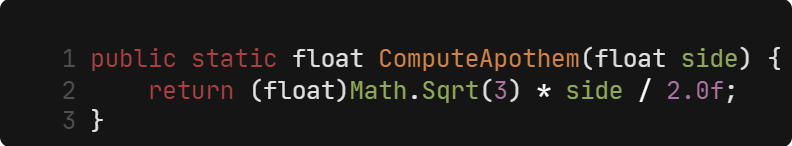
\includegraphics[width=\textwidth]{compute_apothem.png}
                \caption{Calcular apotema del hexágono.}
                \label{fig:compute_apothem}
            \end{figure}

            \begin{figure}[H]
                \centering
                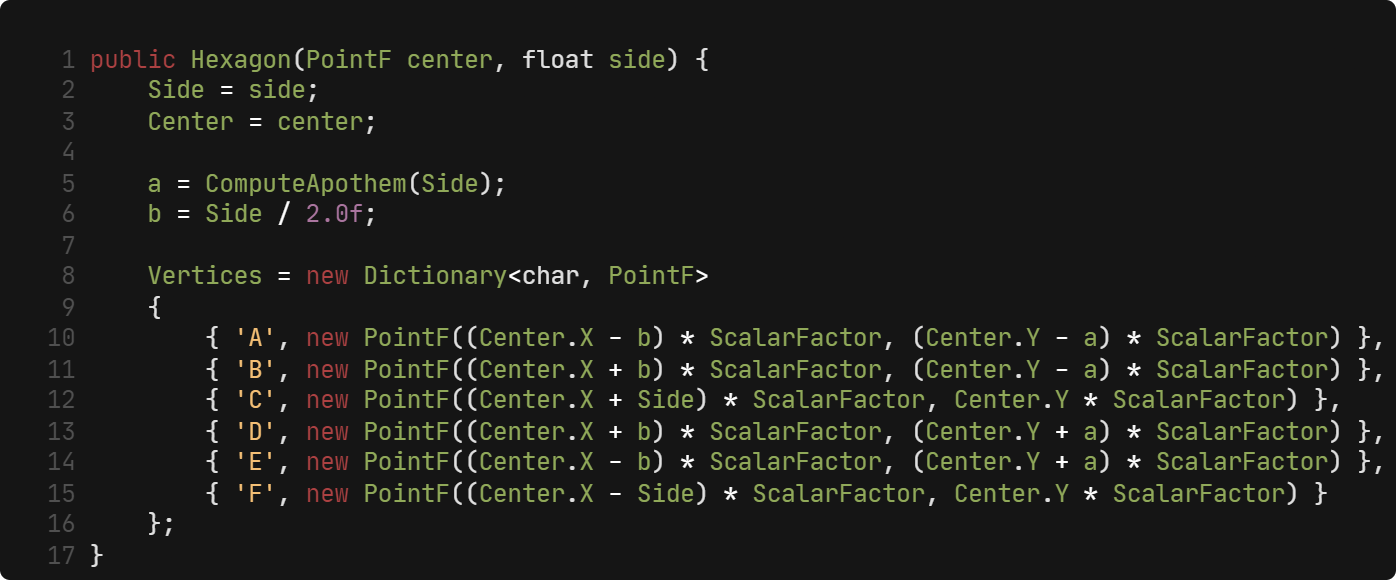
\includegraphics[width=\textwidth]{hexagon_constructor.png}
                \caption{Constructor de la clase \textit{Hexagon}.}
                \label{fig:hexagon_constructor}
            \end{figure}

            \begin{figure}[H]
                \centering
                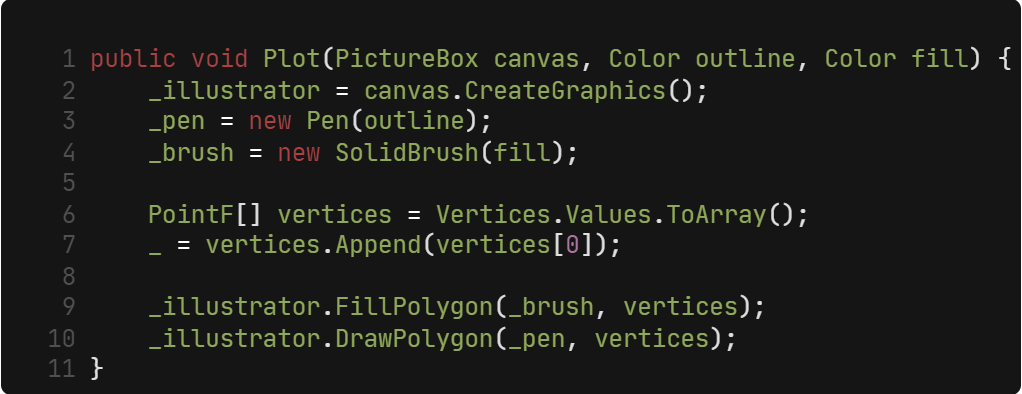
\includegraphics[width=\textwidth]{plot_hexagon.png}
                \caption{Graficar hexágono.}
                \label{fig:plot_hexagon}
            \end{figure}

        \subsection{Clase \textit{BeePanel}}

            \begin{figure}[H]
                \centering
                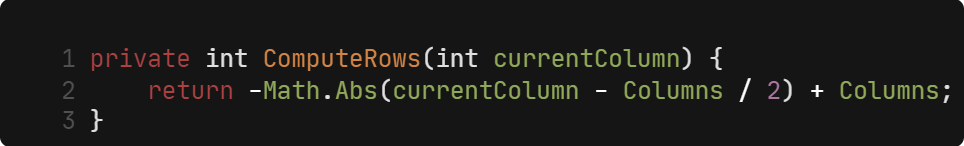
\includegraphics[width=\textwidth]{compute_rows.png}
                \caption{Calcular hexágonos por columna.}
                \label{fig:compute_rows}
            \end{figure}

            \begin{figure}[H]
                \centering
                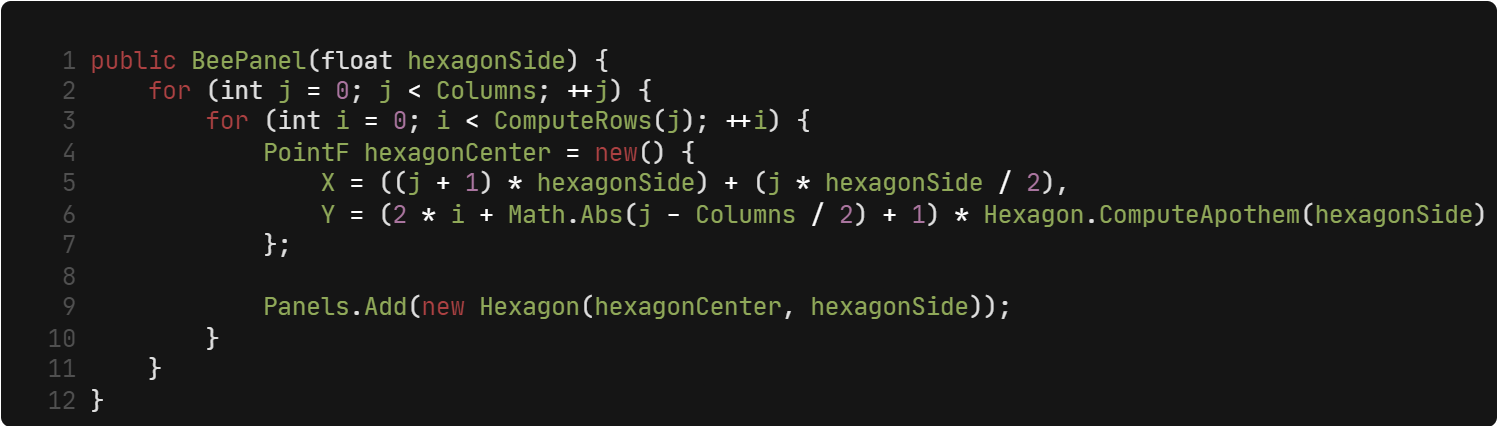
\includegraphics[width=\textwidth]{bee_panel_constructor.png}
                \caption{Constructor de la clase \textit{BeePanel}.}
                \label{fig:bee_panel_constructor}
            \end{figure}

            \begin{figure}[H]
                \centering
                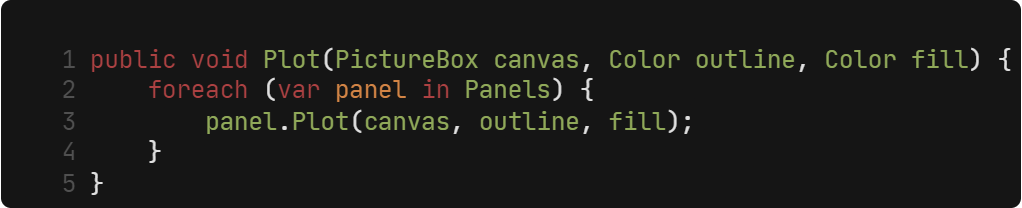
\includegraphics[width=\textwidth]{plot_bee_panel.png}
                \caption{Graficar panal de abejas.}
                \label{fig:plot_bee_panel}
            \end{figure}

        \subsection{Clase \textit{Form1}}

            \begin{figure}[H]
                \centering
                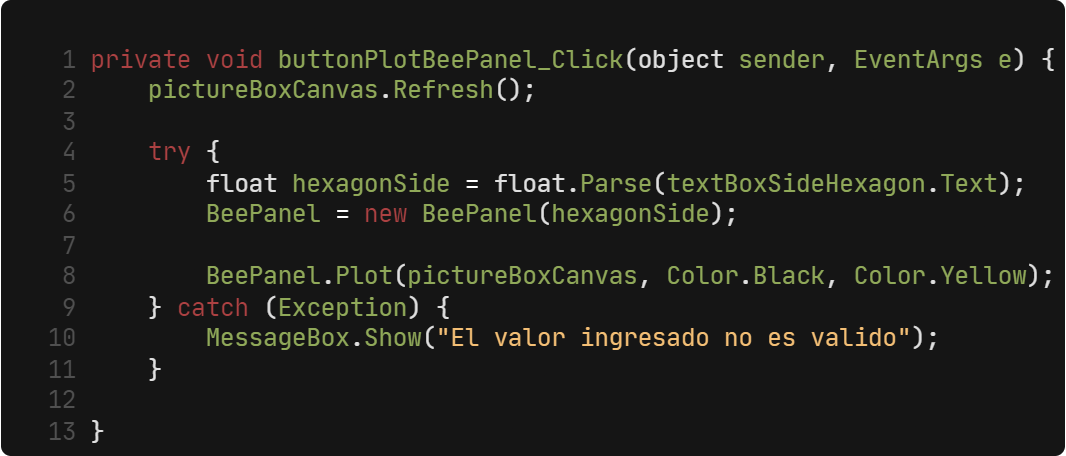
\includegraphics[width=\textwidth]{button_plot_bee_panel.png}
                \caption{Función del botón ``Graficar''.}
                \label{fig:button_plot_bee_panel}
            \end{figure}

    \section{Corrida del programa}
        En la Figura \ref{fig:program_execution} se muestra un ejemplo de la ejecución del programa.

        \begin{figure}[H]
            \centering
            \includegraphics*[width=\textwidth]{program_execution}
            \caption{Dibujado del panal de abejas.}
            \label{fig:program_execution}
        \end{figure}

    \printbibliography

\end{document}